\lhead{\begin{tikzpicture}[remember picture, overlay]
    \node [anchor=100,inner sep=0] (imagenIZQUIERDA) at (current page header area.north){
\includegraphics[width=18cm]{img/Encabezado.PNG}};
    \end{tikzpicture}}
    \rhead{Ángeles-Hurtado}
    \rfoot{\begin{tikzpicture}[remember picture, overlay]
    \node [anchor=140,inner sep=0] (imagenDERECHA) at (current page footer area.south){
\includegraphics[width=18cm]{img/Foot.PNG}};
    \end{tikzpicture}}
    %----------------------------------------------------------------------------------------
    \lfoot{ \thepage}
    % \renewcommand{\labelenumi}{\alph{enumi}.)} 
    %----------------------------------------------------------------------------------------
    %----------------------------------------------------------------------------------------
    %	TITLE SECTION
    %----------------------------------------------------------------------------------------
    
    \setlength{\droptitle}{-5\baselineskip} % Move the title up
    \title{\textbf{Estudio de tiempos y movimientos en el ensamble de un circuito electrónico utilizando diferentes métodos para su optimización }} % Article title
    
     \author{ 
     \textsc{Gómez Hernández, Diego Guadalupe}\\ 
    %  Afiliación:
     \texttt{ Instituto Tecnológico de Querétaro } \\ 
     \texttt{Tecnológico Nacional de México } \\ 
     \texttt{Querétaro, México}\\ 
     \texttt{diego.guadalupe2004@gmail.com} 
     \and 
     \textsc{Ángeles-Hurtado, Luis Alberto}\\ 
    %  Afiliación:
     \texttt{ Instituto Tecnológico de Querétaro } \\ 
     \texttt{ Tecnológico Nacional de México } \\ 
     \texttt{Querétaro, México}\\ 
     \texttt{alb3rt0.ah@gmail.com} 
    }
    
    
    %----------------------------------------------------------------------------------------
    
    % \begin{document}
    
    % Print the title
    \maketitle
    \thispagestyle{fancy}
    
    %----------------------------------------------------------------------------------------
    %	ARTICLE CONTENTS
    %----------------------------------------------------------------------------------------
    
    % \section*{Resumen}
    % \textit{Palabras clave:}
    % El resumen (ancho de página) deberá contener entre 100 y 200 palabras tipo Adobe Devangari 11 puntos.
    
    \begin{abstract}
    \noindent 
    El resumen (ancho de página) deberá contener entre 100 y 200 palabras tipo Adobe Devangari 11 puntos.
    
    \end{abstract}
    % 
    % 
    \textbf{\textit{Palabras clave}}: {First keyword should be the corresponding to the research area according with the authors guide. Maximum of 6 keywords.}
    % \keywords{First keyword should be the corresponding to the research area according with the authors guide. Maximum of 6 keywords.}
    
    \section{Introducción}
    
    
    \begin{itemize}
    
        \item Define estudio de tiempos y movimientos: Se refiere a examinar los métodos, materiales, herramientas e instalaciones empleadas o por emplear en la realización de una tarea específica.\cite{neira2006tecnicas}
        \item Define que es ensamble: Se trata de unir, ensamblar o ajustar una pieza con otra\cite{Ensamble}
        \item Define que es circuito electrónico: Este se compone de placas que contienen materiales semiconductores, así como componentes activos y pasivos. Su objetivo es establecer un camino continuo por el cual pueda circular la corriente eléctrica. Se basa en el movimiento de electrones para generar, transmitir, recibir y almacenar información.
        \item Define el método de tiempos predeterminados: Es el conjunto de reglas o métodos que determinan los movimientos. \cite{freivalds2014ingenieria}
        \item Define optimización: Encontrar la manera mas rápida y efectiva de hacer una tarea. \cite{optimización}
        
        \item Incrementar la eficiencia del ensamble del circuito reduciendo el tiempo necesario, logrando así una mejora en su proceso para hacerlo más efectivo y productivo.
        \item Algunas metodologías más comunes para analizar la eficiencia laboral se encuentran la metodología Ágil, el modelo de cascada y diversos sistemas de medición de tiempos como MTM, GPD, BMT y MODADPTS. Estos enfoques facilitan la evaluación y medición de las técnicas empleadas para calcular el tiempo que un empleado dedica a realizar una tarea específica.\cite{freivalds2014ingenieria}
        \item El principal propósito del estudio de trabajo es elevar la eficiencia sin necesidad de grandes inversiones y siempre buscando la forma mas económica de hacerlo. Se pretende mejorar el rendimiento mediante la optimización del trabajo, que por lo general implica costos mínimos.
        \item Definamos estudio del trabajo a ciertas técnicas, y en particular estudio de métodos y medida del trabajo, que se utilizan para examinar el trabajo humano en todos sus contextos y que llevan sistemáticamente a investigar todos los factores que influyen en la eficacia y en la economía de la que estudiada, con el fin de mejorarla. 
        \cite{neira2006tecnicas}
        
    \end{itemize}
    % 
    % 
    \section{Justificación}
    
    \begin{itemize}
        \item El proyecto actual se enfocará en examinar, mejorar e integrar sistemas de producción de bienes y servicios mediante la aplicación de tecnologías para aumentar la eficiencia y medir el rendimiento. Este trabajo permitirá la aplicación de varios enfoques, como el análisis de tiempos y movimientos, para mejorar y perfeccionar el montaje de un circuito electrónico.
        \cite{freivalds2014ingenieria}
    \end{itemize}
    % 
    % 
    \section{Descripción del problema}
    \begin{itemize}
        \item Se trata de optimizar un procedimiento para que sea más sencillo tanto para el trabajador como para el analista, logrando un resultado efectivo. Esto implica considerar el tiempo que el trabajador tarda en realizar la tarea y poder analizar los datos correspondientes.
        \item Es necesario emplear diversos enfoques de estudio del trabajo, teniendo en cuenta las distintas variables que surjan, con el fin de determinar el método más adecuado para el proceso de ensamblaje.
    \end{itemize}
    
    
    % 
    % 
    \section{Fundamentación teórica}
    
    
    \begin{itemize}
        \item Incrementar la eficiencia del ensamblaje de circuitos electrónicos es crucial en la industria moderna para mantener la competitividad y la calidad del producto. Este objetivo se logra reduciendo el tiempo necesario para el ensamblaje, lo que a su vez mejora la efectividad y la productividad del proceso.
        \item El estudio del trabajo es fundamental para elevar la eficiencia en el ensamblaje de circuitos electrónicos. Este consiste en un conjunto de técnicas, incluido el estudio de métodos y la medición del trabajo, que se utilizan para examinar el trabajo humano en todos sus contextos. El objetivo es investigar todos los factores que influyen en la eficacia y la economía del proceso de ensamblaje, con el fin de mejorarlos de manera continua.\cite{estudio_del_trabajo}
        \item  La optimización del ensamblaje requiere un enfoque integral que incluya la aplicación de metodologías de eficiencia laboral, el estudio del trabajo y la identificación de áreas de mejora en el proceso de ensamblaje. Este enfoque permite reducir el tiempo necesario para el ensamblaje, mejorar la efectividad y la productividad del proceso, y garantizar la calidad del producto final.
        \cite{freivalds2014ingenieria}
    \end{itemize}
    % 
    % 
    \section{Hipótesis}
    
    Es la suposición con fundamento científico relativa a la solución del problema, necesidad o de cómo se aprovecha la oportunidad con la incógnita científica y se fundamenta con: 1. Una suposición (en afirmativo o negativo) y ésta deberá vincularse con:
    2. La fundamentación científica que deberá ser precisa 3. Una entidad de comparación para probar la suposición y
    4. La variable con que se califica o cuantifica la comparación o se prueba la hipótesis.
    
    \begin{itemize}
        \item Se debe de identificar claramente la suposición científica
        \item Se debe de identificar claramente el fundamento científico
        \item Se debe identificar claramente la variable de respuesta
        \item Se debe identifican claramente las realidades o modelos contrastantes
        \item Se debe de establecer las variables asociadas, explicativas o que tienen relación funcional con la variable de respuesta
    \end{itemize}
    % 
    % 
    \section{Objetivo}
    
    \begin{itemize}
        \item Diseña, mejora e integra sistemas productivos de bienes y servicios aplicando tecnologías para su optimización. 
        \item Diseña, implementa y mejora sistemas de trabajo para elevar la productividad.
        \item Mejorar el proceso de ensamble haciéndolo más rápido y económico, eliminando pasos innecesarios y buscando formas más eficientes de realizarlo, sin comprometer la calidad del ensamble. 
    \end{itemize}
     
    
    \subsection{Objetivos específicos }
    
    \begin{itemize}
        \item Aplicar las técnicas de estudio de tiempos y movimiento.
        \item Aplicar la medición de tiempos y métodos (MTM).
        \item Diseñar y elaborar un instructivo claro y conciso sobre el ensamble del circuito. 
    \end{itemize}
    
    % 
    % 
    \section{Cuerpo (Metodología, modelo matemático, etc.)}
    
        \begin{table}[H]
        \huge
        \tiny
        \begin{tabular} {|c|c|c|}
        \hline
        \multicolumn{3}{|c|}{MATERIALES} \\
        \hline 
        NOMBRE & CANTIDAD & PLANO\\
        \hline
        CABLE MH & 9 & 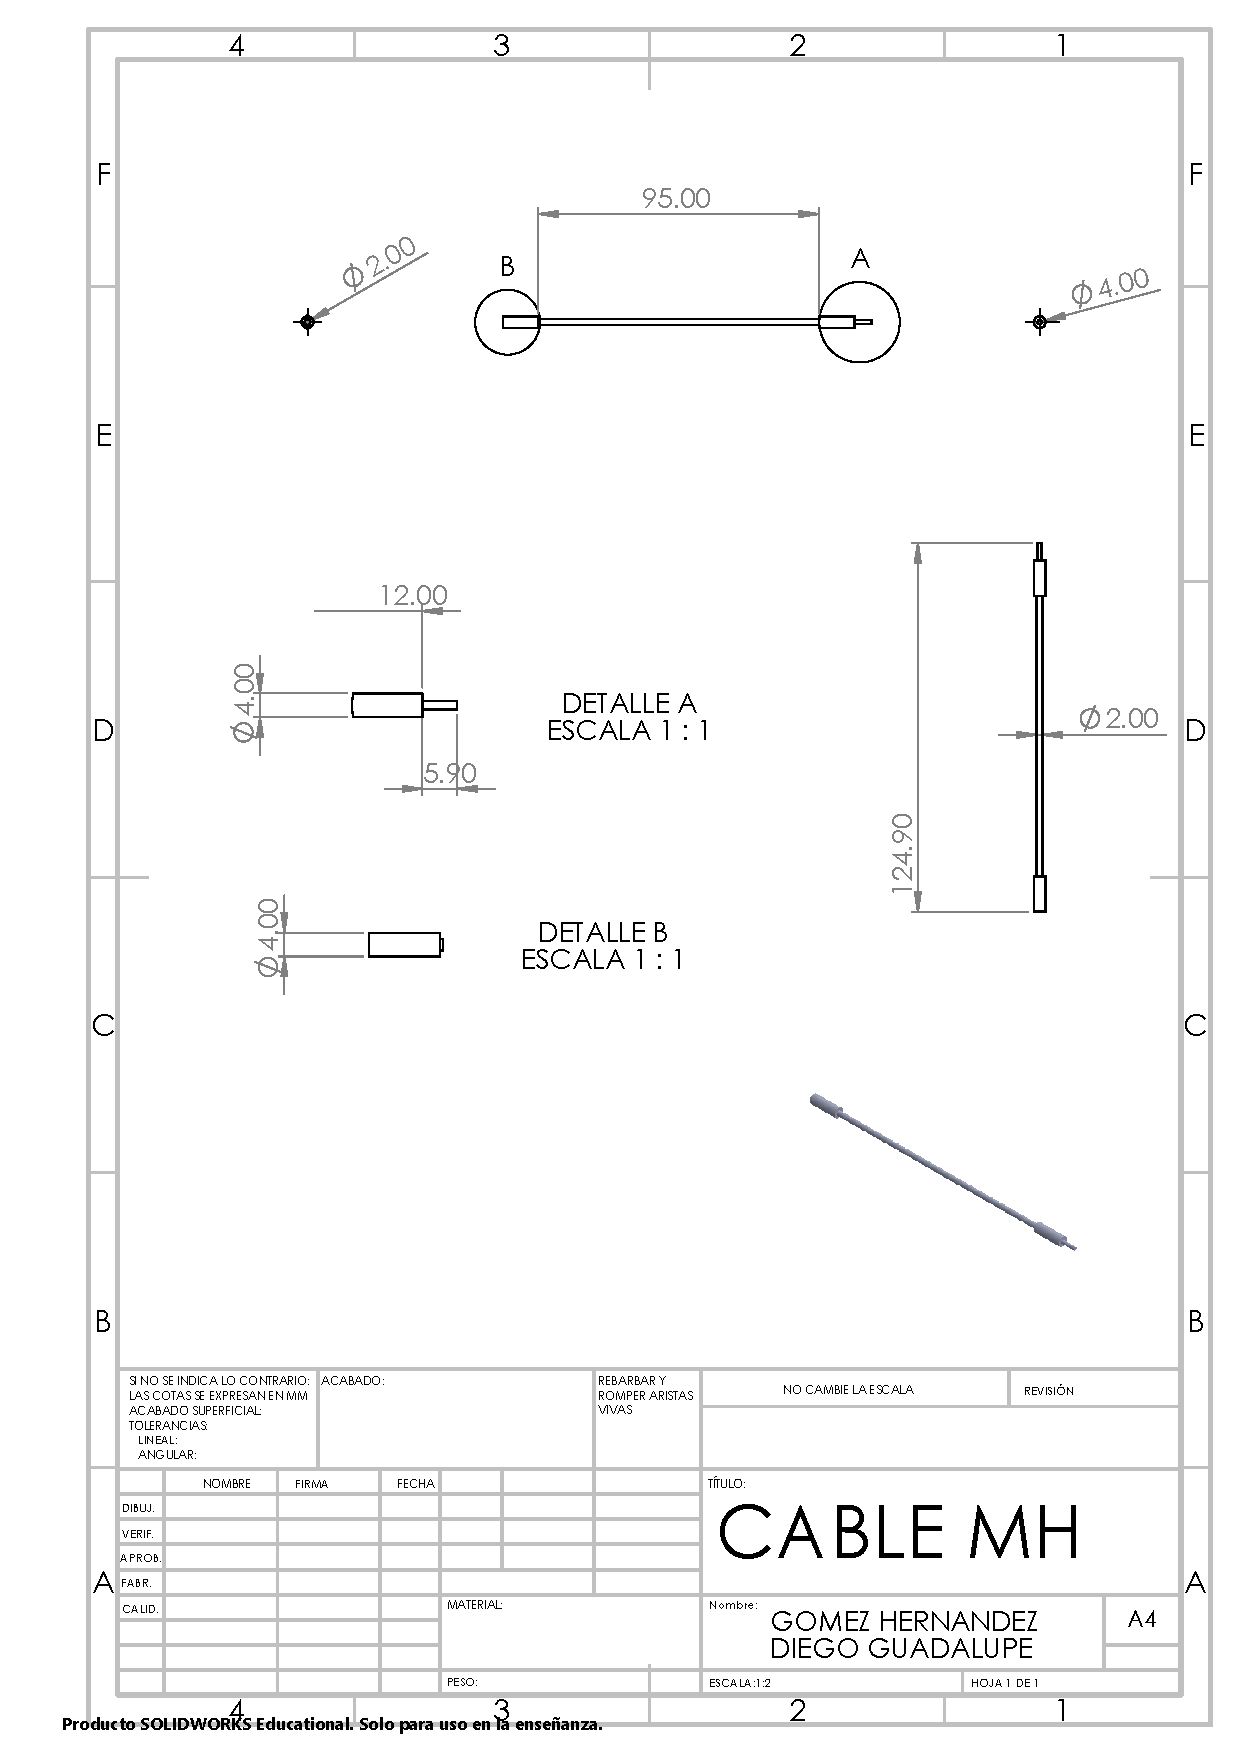
\includegraphics[width=19mm]{13/img/PlanoCableMh.pdf} \\
        \hline
        CABLE MM & 4 & 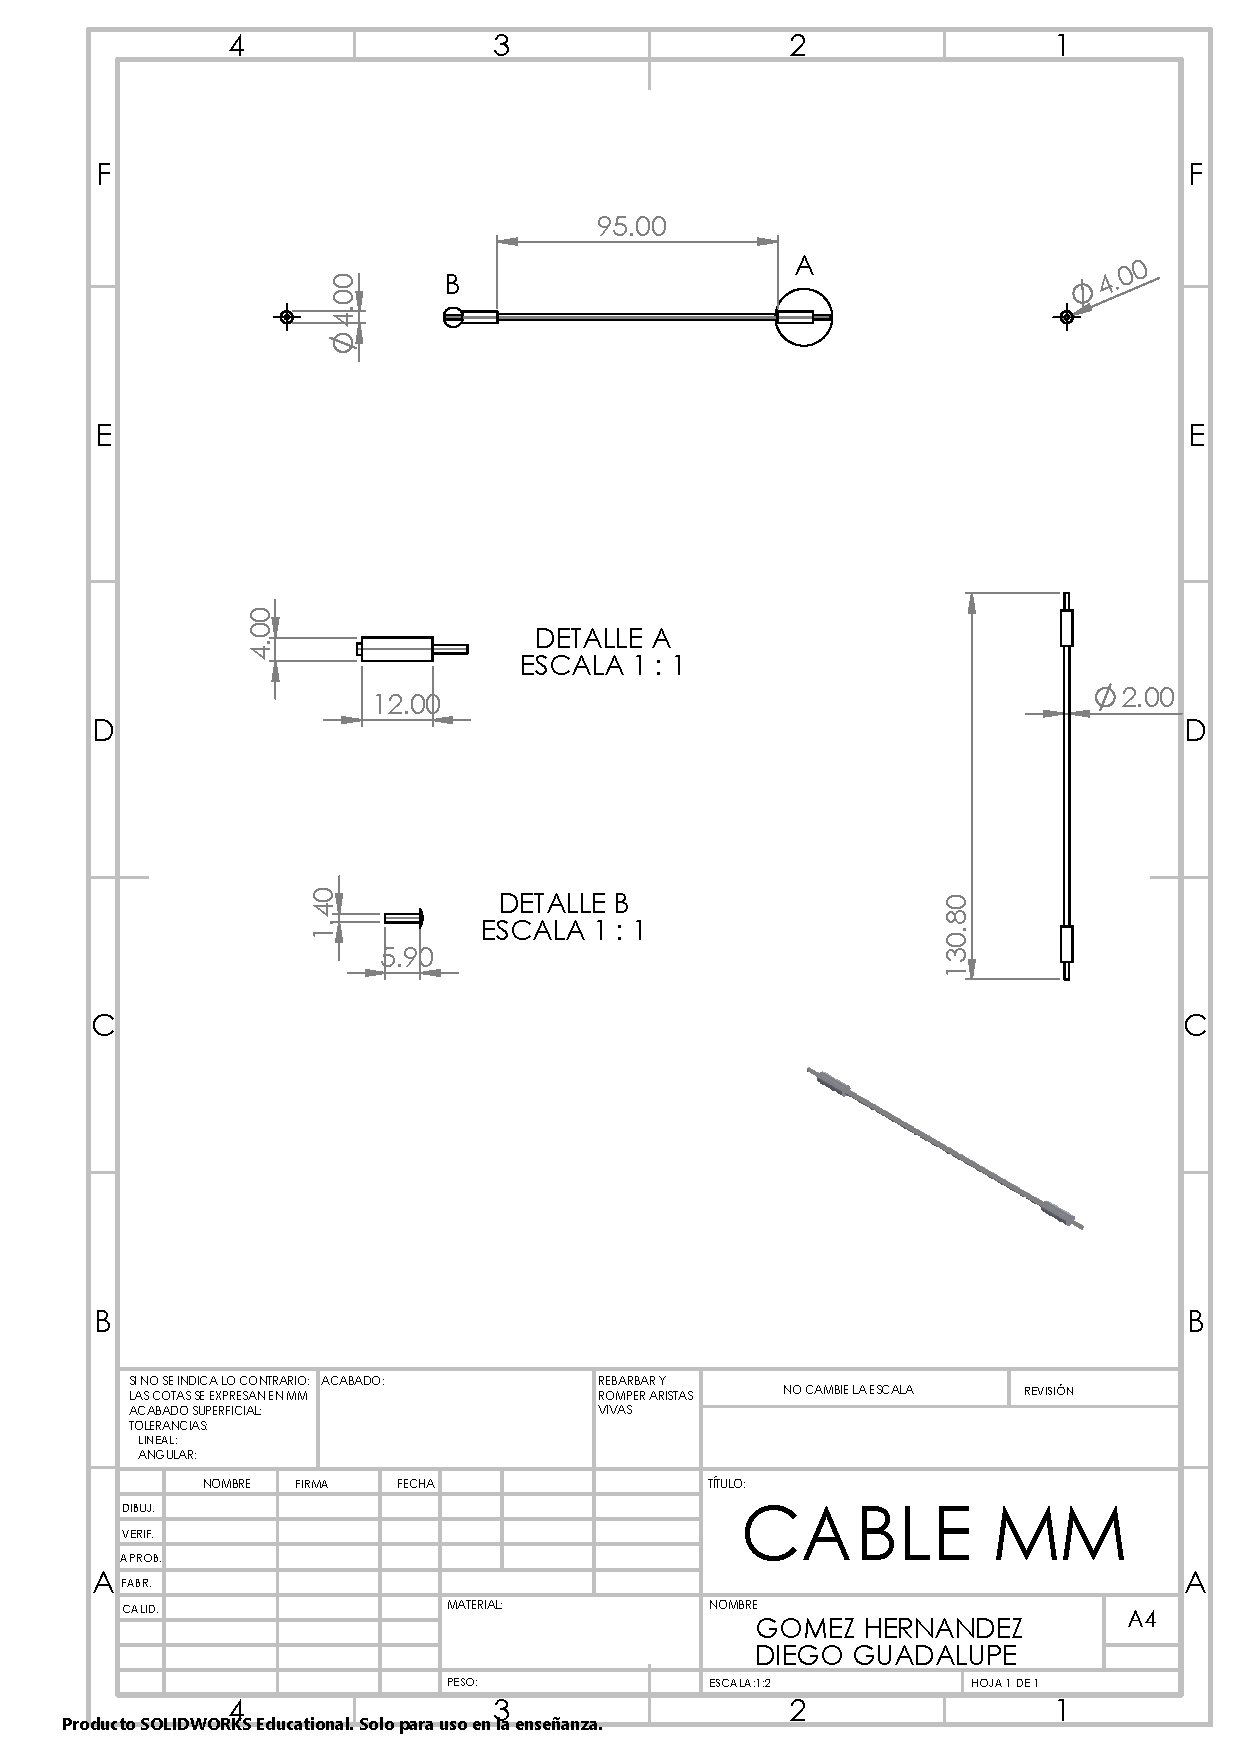
\includegraphics[width=19mm]{13/img/PlanoCableMm.pdf}\\
        \hline
        RESISTENCIA & 2 & 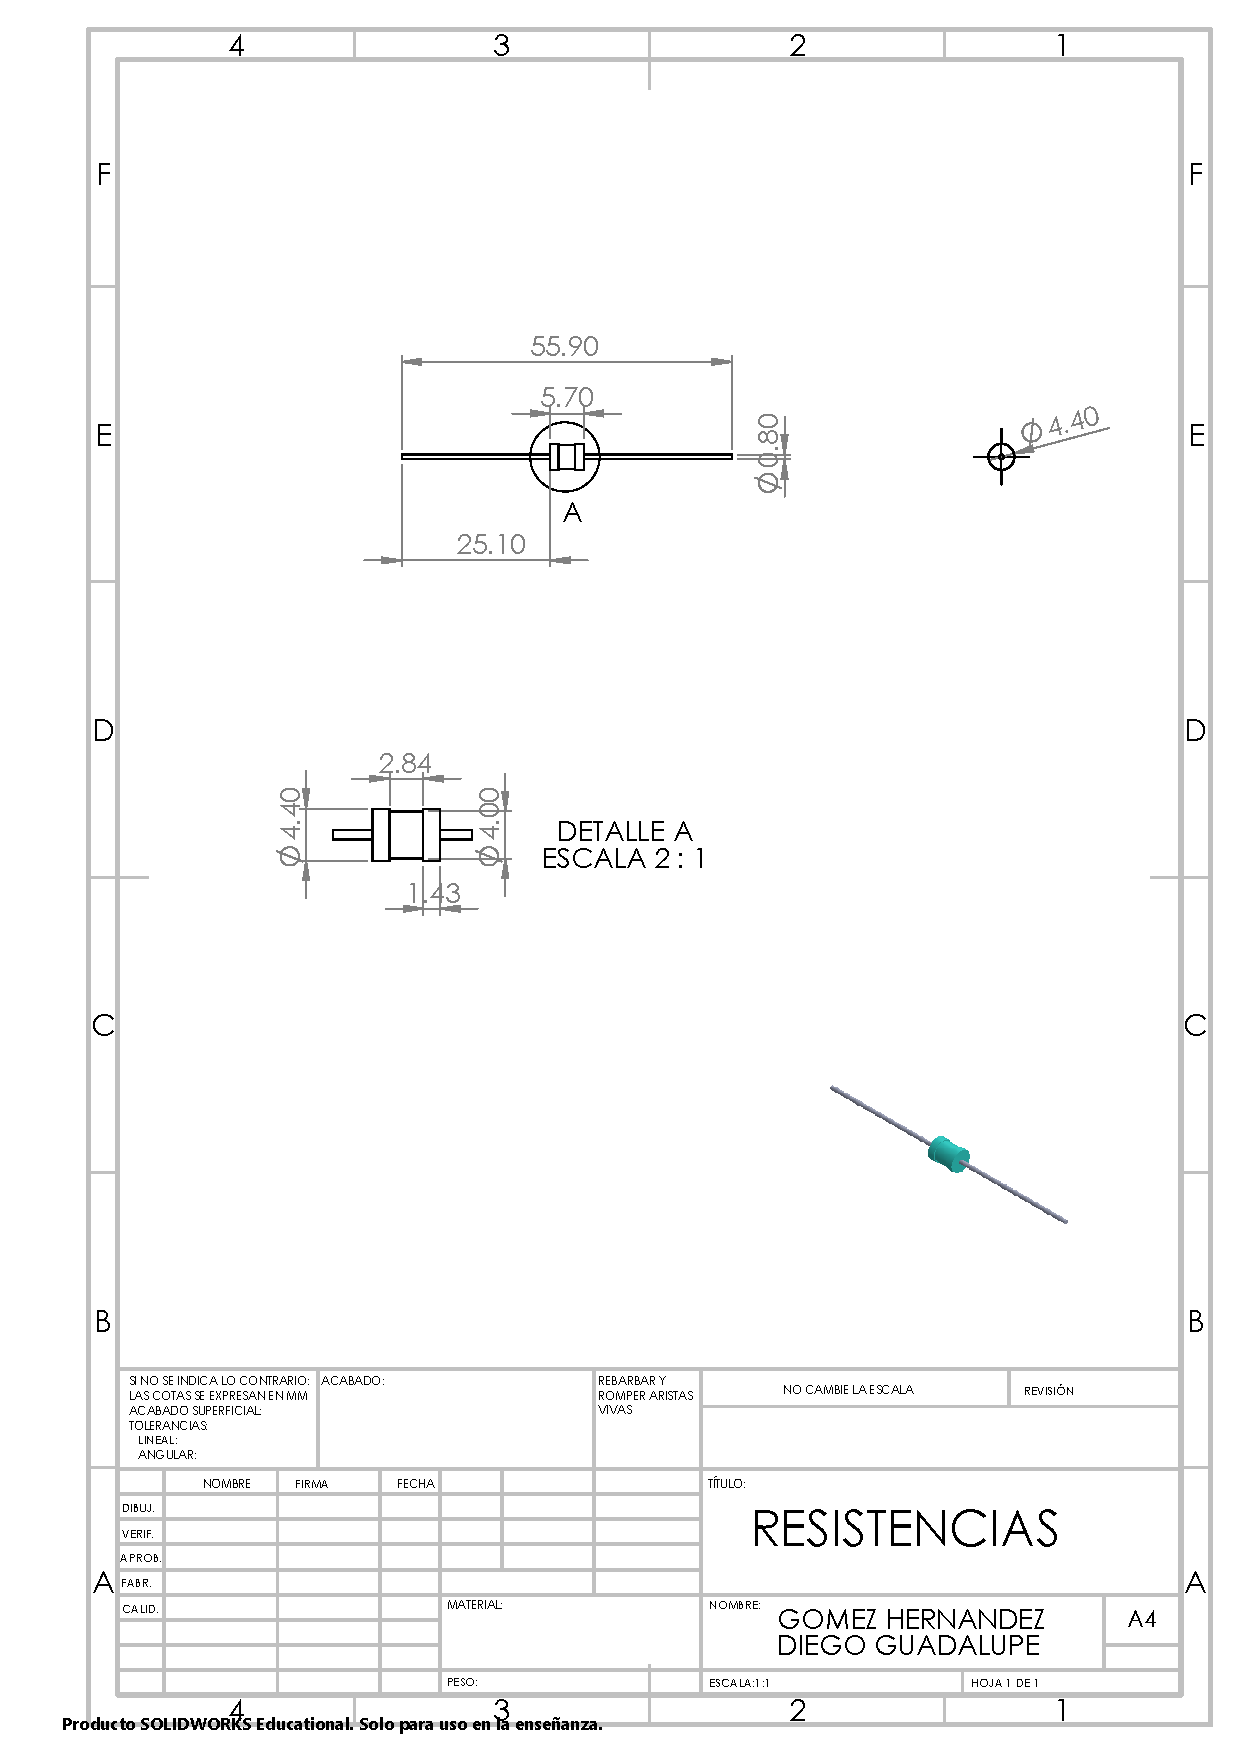
\includegraphics[width=19mm]{13/img/PlanoResistencia.pdf}\\
        \hline
        LCD & 1 & 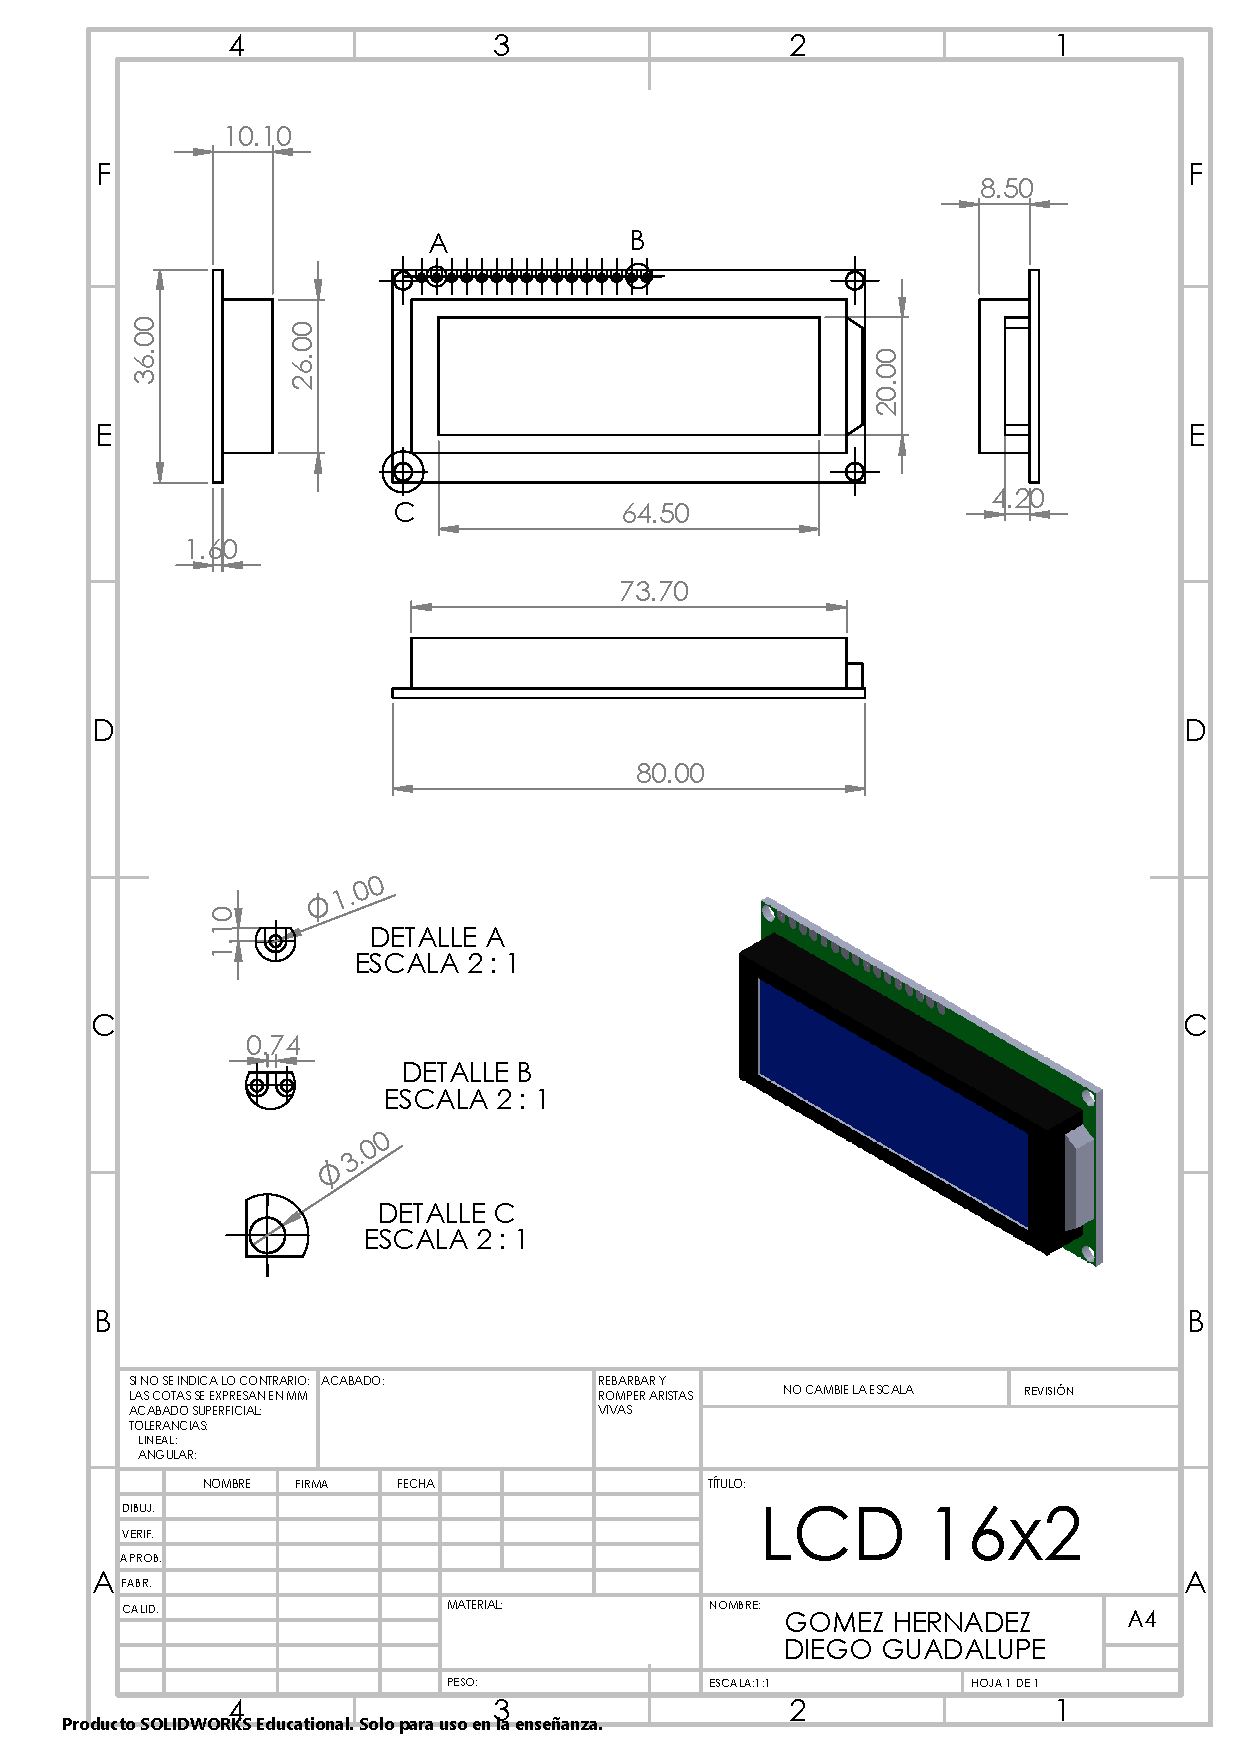
\includegraphics[width=19mm]{13/img/PlanoLcd.pdf}\\
        \hline
        ESP & 1 & 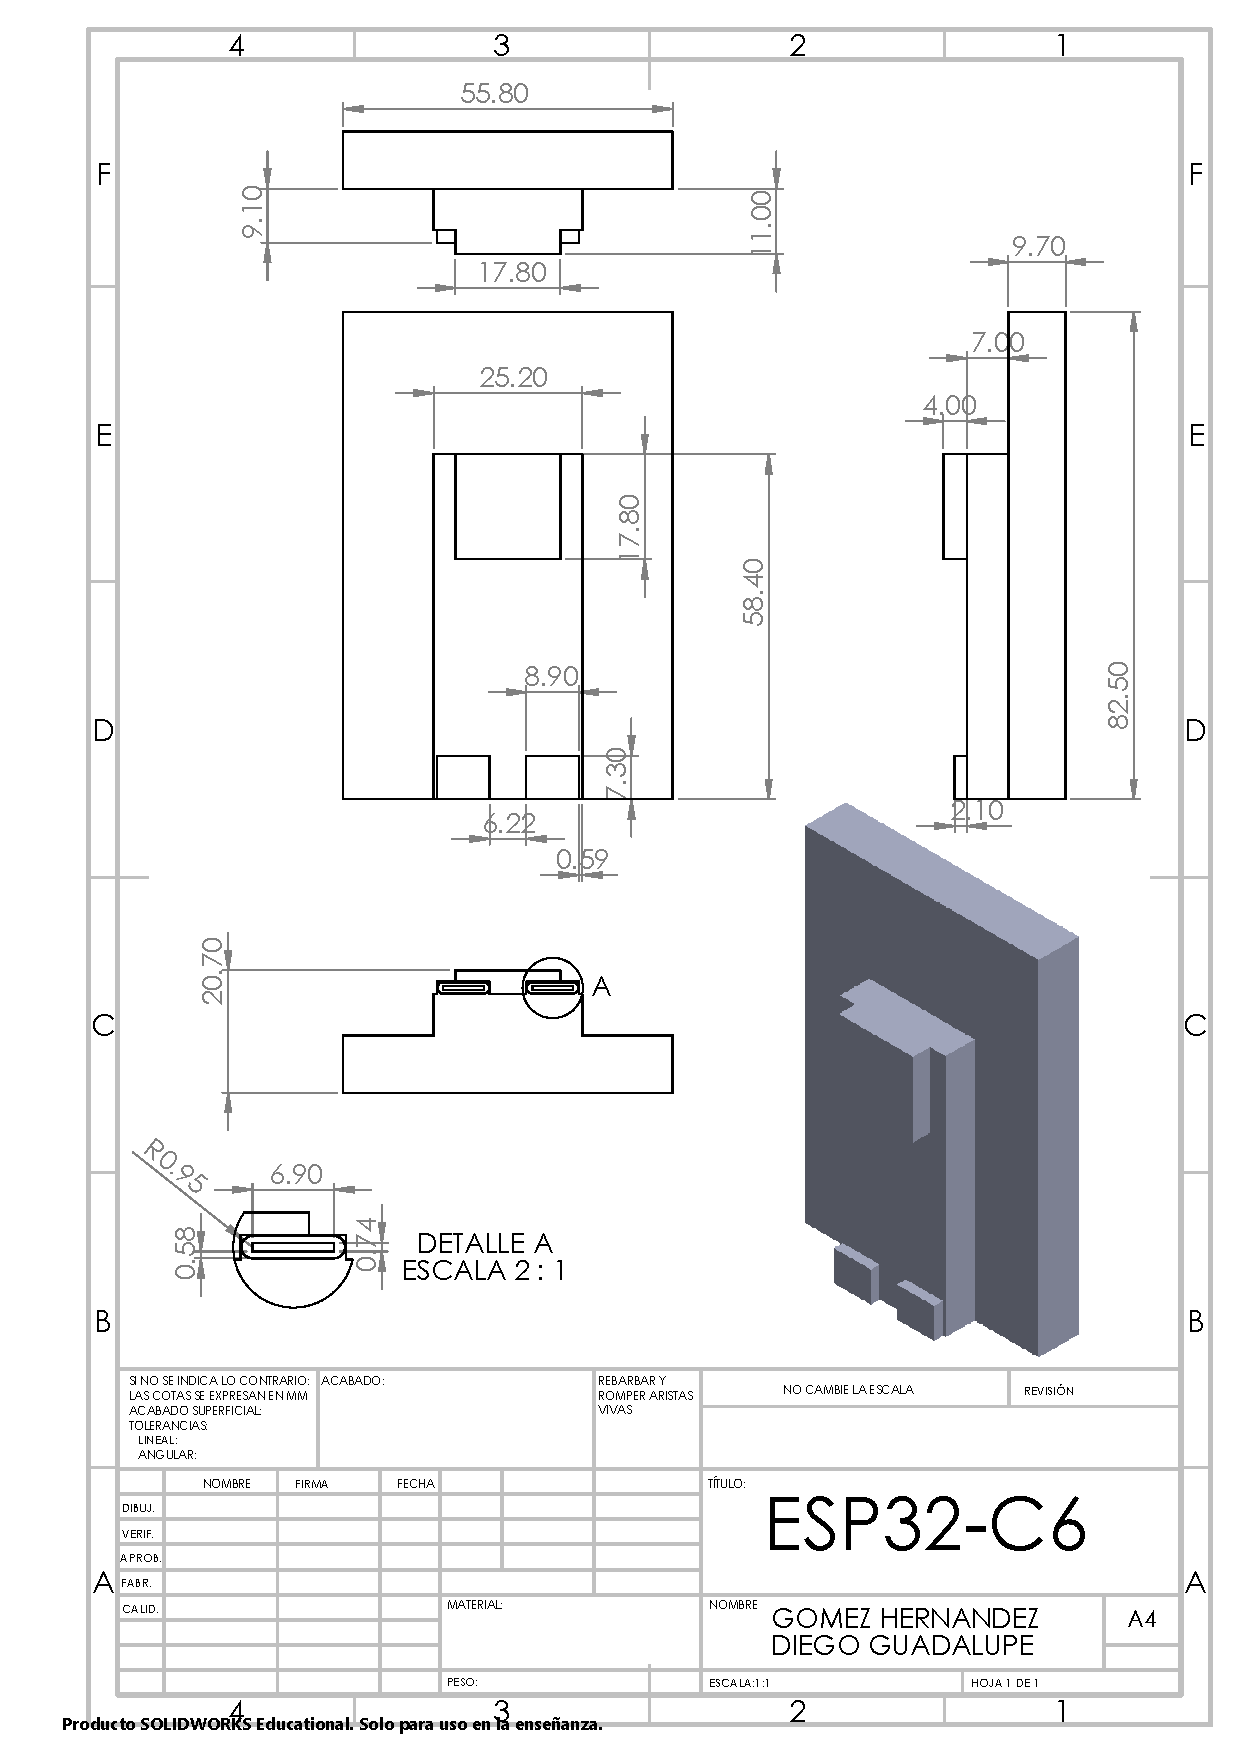
\includegraphics[width=19mm]{13/img/PlanoEsp.pdf}\\
        \hline
         POTENCIOMETRO & 1 & 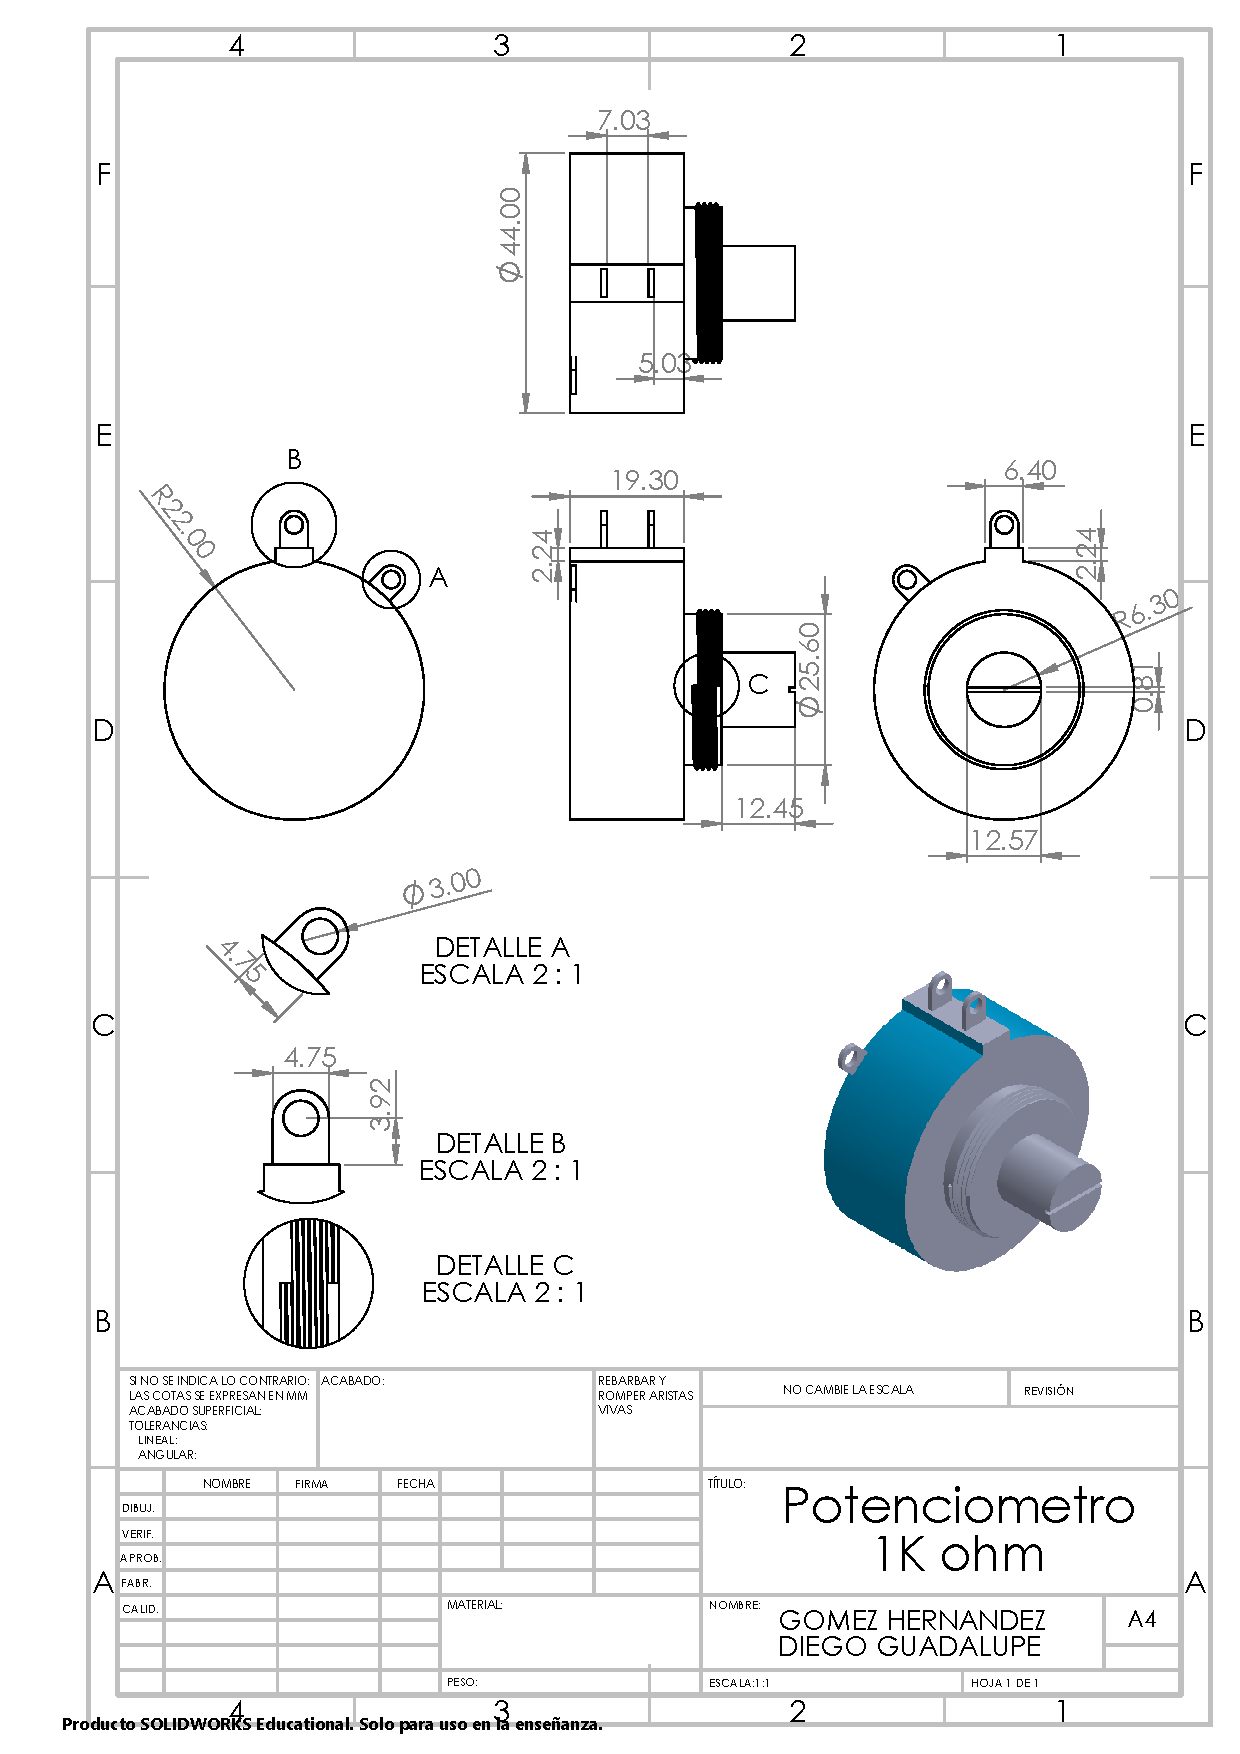
\includegraphics[width=19mm]{13/img/PlanoPotenciometro.pdf}\\
        \hline
        \end{tabular}
        \caption{TABLA DE MATERIALES}
        \label{tab:my_label}
    \end{table}
    
         Visualización de los planos:
    \begin{itemize}
        \item CABLE MH \ref{anexo:PlanoCableMh}
        \item CABLE MM \ref{anexo:PlanoCableMm}
        \item ESP32-C6 \ref{anexo:PlanoEsp}
        \item LCD 16x2 \ref{anexo:PlanoLcd}
        \item Potenciometro 1K ohm \ref{anexo:PlanoPotenciometro}
        \item RESISTENCIAS \ref{anexo:PlanoResistencia}
    \end{itemize}
    
        Una vez teniendo los materiales necesarios accederemos al manual que se encuentra en la siguiente referencia.
        \ref{anexo:ensambleCircuitoElectrónicoESP32-C6.pdf}
    
        Después de leer el manual podremos iniciar el ensamble del circuito electrónico el cual nos servirá para tomar tiempos y poder seguir con nuestro proyecto. 
    
    % 
    %
    % 
    % 
    \subsection{Prepara tu documento}
    
    Antes de que comiences a utilizar esta plantilla, es recomendable que prepare la información que contendrá en un archivo aparte. 
    Ten preparadas tus gráficas, así como también las tablas aparte, para que sea más fácil integrarlo. 
    Se recomienda fuertemente el uso de \textbf{formato Enhanced Metafile (.emf) para imágenes y gráficas} de resolución óptima. 
    Finalmente, completa y organiza el contenido antes de darle el formato de esta plantilla. 
    
    \subsection{Acrónimos y Abreviaciones}
    
    Los acrónimos y abreviaciones deberán ser definidos únicamente la primera vez que aparecen en el texto, esto para que el lector entienda lo que significan.
    
    \subsection{Ecuaciones}
    
    Las ecuaciones son una excepción a las especificaciones prescritas de esta plantilla. 
    Deberá determinar si su ecuación debe escribirse o no utilizando la fuente Adobe Devangari. 
    Para crear ecuaciones multinivel, puede ser necesario tratar la ecuación como un gráfico e insertarla en el texto después de aplicar el estilo de la platilla.
    Las ecuaciones serán enumeradas de manera consecutiva, y el número de ecuación, entre paréntesis, se colocan al ras de la derecha, utilizando una tabulación derecha. 
    
    \begin{equation}
        \label{eq1}
        x + y = z 
    \end{equation}
    
    Es importante asegurarse de que los símbolos de la ecuación sean definidos antes o inmediatamente después de la ecuación. Utilice “(1)”, en vez de “Eq. 1” al enumerar las ecuaciones, excepto al principio de una oración: “La ecuación (\ref{eq1}) es…”
    
    \section{Resultados y discusión}
    
    Antes de comenzar a preparar tu artículo, es importante que lea primero la guía del autor, la cual incluye los temas o apartados que son necesarios para tener tu trabajo completo.
    Una vez completada la edición del texto, el documento está listo para el uso de esta plantilla. En este archivo recién creado, resalte todo el contenido e importe el archivo de texto preparado. Ahora esta listo para estilizar su documento.
    En esta sección se deben presentar todo lo obtenido de la sección 2, incluidas deducciones o efectos del desarrollo. También se podrán incluir subsecciones numeradas de la siguiente forma:
    
    \subsection{Autores y Afiliaciones}
    
    Para distinguir las afiliaciones de los autores, utilice superíndices iniciando con el número 1, 2, etc., sucesivamente, esto dependerá de la cantidad de los departamentos a los que estén afiliados los autores. En caso de que todos los autores pertenezcan a una mismo departamento e institución, utilizar sólo el superíndice 1. 
    
    \subsection{Identificar los encabezados}
    
    Se les recuerda a los autores que los encabezados deben de estar conforme los solicita la guía del autor. De ahí se puede adaptar el trabajo para que sea más fácil de entender para el lector.
    Los encabezados organizan los temas sobre una base relacional y jerárquica. Por ejemplo, el título del documento es encabezado del texto principal porque todo el material posterior se relaciona y elabora sobre este tema. 
    
    \subsection{Tablas y Figuras}
    
    \begin{enumerate}
        \item Posición de las tablas y figuras: Coloque las figuras y las tablas en la parte superior e inferior de las columnas. Evite colocarlos en medio. Las figuras y las tablas grandes pueden abarcar ambas columnas. Los títulos de las figuras deben de estar debajo de las mismas; los títulos de las tablas deben aparecer encima de ellas. Insértese las figuras y los cuadros después de citarse en el texto. Utilice la abreviatura “Fig. 1”, incluso al principio de una oración. 
    \end{enumerate}
    
    \section{Conclusiones}
    
    Se describe aquí el alcance del trabajo, logros obtenidos y perspectivas para el futuro de este. Se sugiere colocar información cuantitativa obtenida.
    
    \section{Agradecimientos}
    
    Es importante darles su debido reconocimiento a los laboratorios, instituciones, organizaciones, entre otros que han sido participes para la culminación de este trabajo. También es importante mencionar, fondos, proyectos, becas, entre otros que se le han otorgado al o los autores para realizar el trabajo de investigación. Ejemplo: “Los autores agradecen al Concejo Nacional de Ciencia y Tecnología por los recursos otorgados…”
    
    \section*{Referencias}
    
    Para esta platilla, se solicita al autor enumerar las citas de manera consecutiva entre corchetes . 
    La puntuación de la oración que sigues sería . 
    Refiérase simplemente al número de referencia, como en , no utilice “Ref. [3]” o “referencia [3]” excepto al principio de una oración: “La referencia [3] fue la primera…”
    Enumere las notas al pie por separado en superíndices. Coloque la nota de pie de en la parte inferior de la columna en la que se citó. No coloque notas al pie en la lista de referencias. Utilice letras para las notas al pie de la tabla.
    A menos de que haya tres autores o más; no utilice “et al.”. Los trabajos que no hayan sido publicados, incluso si han sido presentados para su publicación, deben ser citados como “inéditos”. Los trabajos que han sido aceptados para su publicación deben de citarse como “en prensa”. Poner en mayúscula sólo la primera palabra de un título, excepto los nombres propios y los símbolos de elemento. 
    
    
    % Ejemplo
    %  @Article{article,
    % 	author = "Author1 LastName1 and Author2 LastName2 and Author3 LastName3",
    % 	title = "Article Title",
    % 	volume = "30",
    % 	number = "30",
    % 	pages = "10127-10134",
    % 	year = "2013",
    % 	doi = "10.3389/fnins.2013.12345",
    % 	URL = "http://www.frontiersin.org/Journal/10.3389/fnins.2013.12345/abstract",
    % 	journal = "Frontiers in Neuroscience"
    % }
    
    % @book{book,
    %   author    = {Author Name}, 
    %   title     = {The title of the work},
    %   publisher = {The name of the publisher},
    %   address   = {The city},
    %   year      = 1993,
    % }
    
    % @incollection{chapter,
    %   author       = {Bauthor Surname}, 
    %   title        = {The title of the work},
    %   editor       = {Editor Name},
    %   booktitle    = {The title of the book},
    %   publisher    = {The name of the publisher},
    %   address      = {The city},
    %   year         = 2002,
    %   pages        = {201-213},
    % }
    
    % @InProceedings{conference,
    %   author = {Cauthor Name and Dauthor Surname and Fauthor LastName},
    %   title = {The title of the work},
    %   booktitle = {The title of the conference proceedings},
    %   year = 1996,
    %   publisher = {The name of the publisher},
    %   editor = {Editor Name1 and Editor Name2},
    %   pages = {41-50},
    % }
    
    % @book{cho,
    %   author       = {Gauthor Name1}, 
    %   title        = {The title of the work},
    %   publisher = {Country code and patent number},
    %   address      = {Patent Country},
    %   year = 2013
    % }
    
    % @book{patent,
    %   author    = {Hauthor Surname1}, 
    %   title     = {The title of the work},
    %   publisher = {Patent number},
    %   address   = {Patent country},
    %   year      = 2010,
    % }
    
    % % please use misc for datasets
    % @misc{dataset, 
    % 	author = "Author1 LastName1 and Author2 LastName2 and Author3 LastName3",
    % 	title = "Data Title",
    % 	year = "2011",
    % 	doi = "10.000/55555",
    % 	URL = "http://www.frontiersin.org/",
    % }
    
    \bibliographystyle{ieeetr}
    \bibliography{13/referencias}
    % 
    % 
    %%%%%%%%%%%%%%%%%%%%%%%%%%%%%%%%%%
    \appendix
    %%%%%%%%%%%%%%%%%%%%%%%%%%%%%%%%%%
    % 
    % 
    \newpage
    \centering{\section[\appendixautorefname{}]{APÉNDICE}}\label{anexo:PlanoCableMh}
    \includepdf[pages=-]{13/img/planoCableMh.pdf}
    %
    \centering{\section[\appendixautorefname{}]{APÉNDICE}} \label{anexo:PlanoCableMm}
    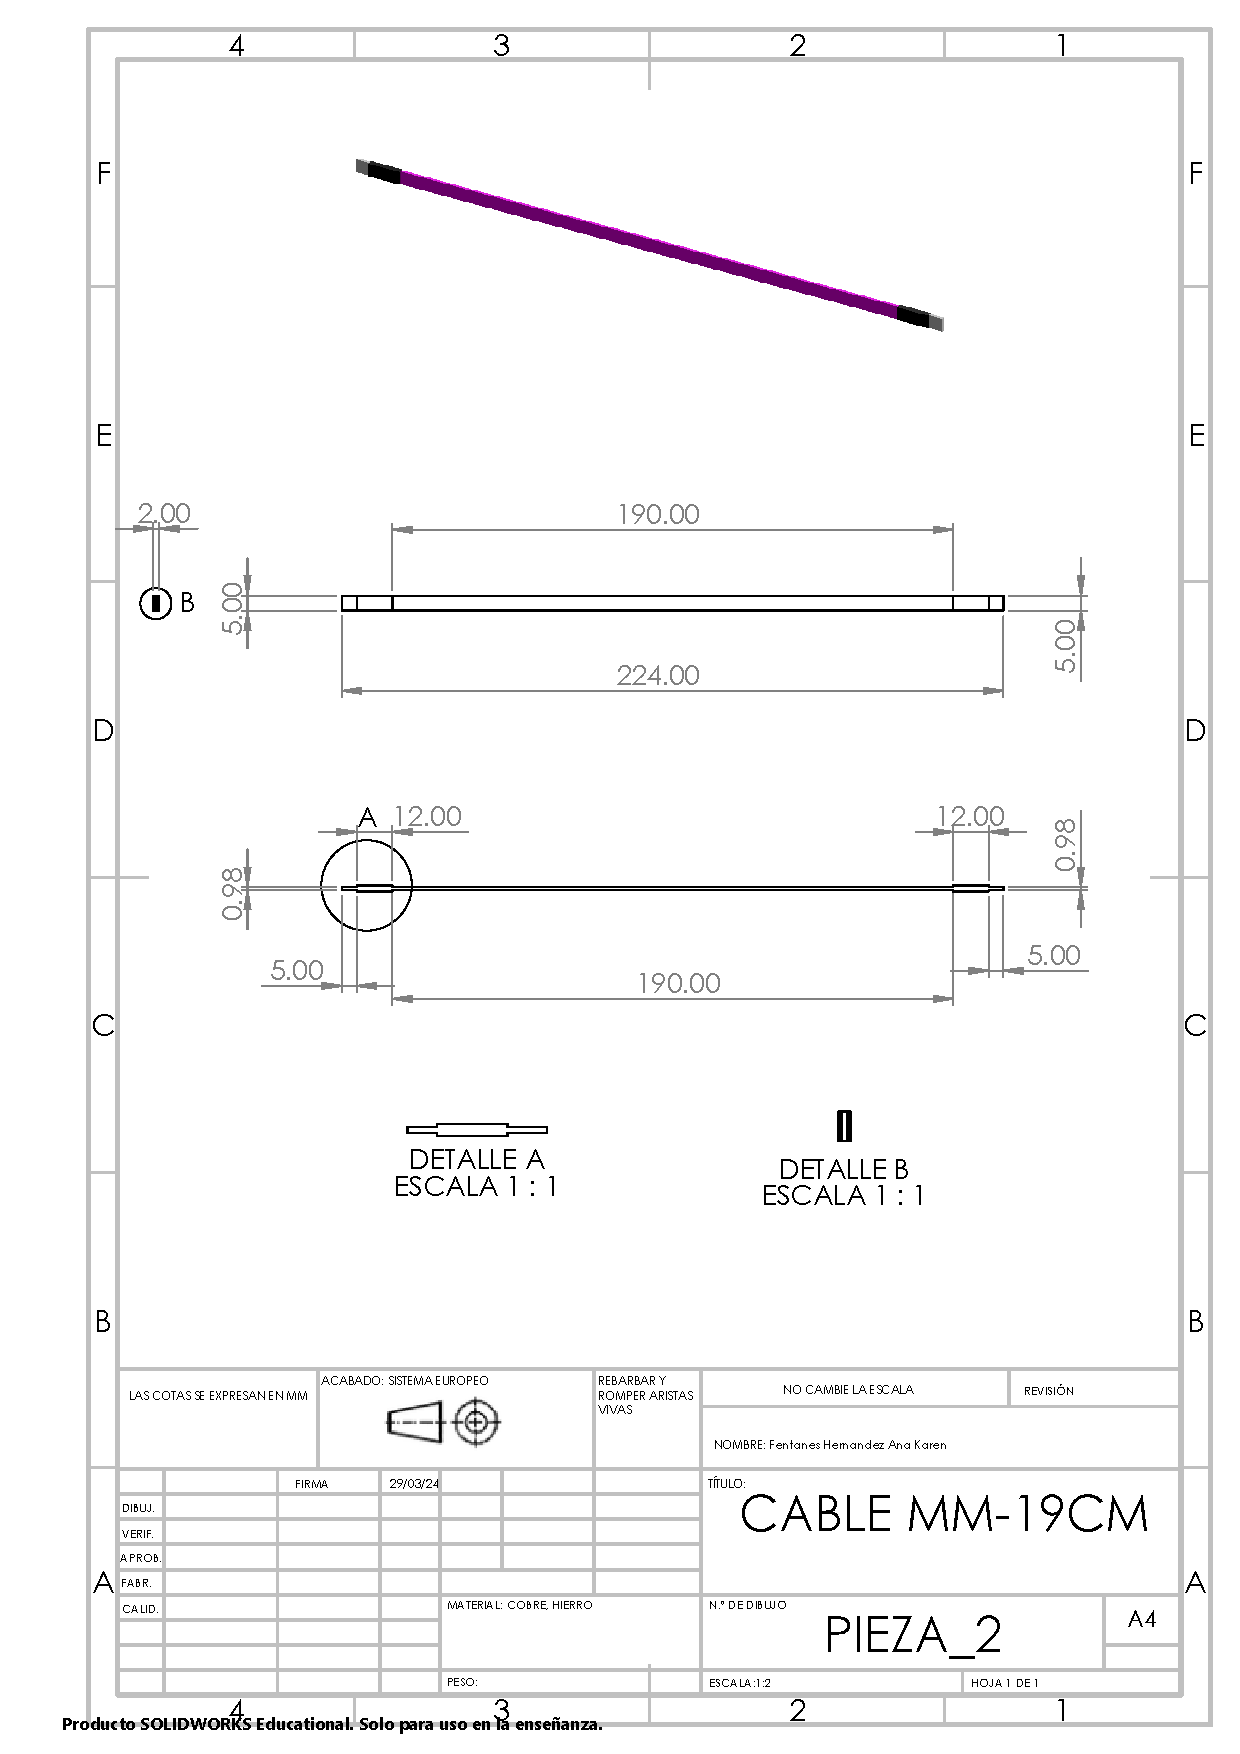
\includepdf[pages=-]{13/img/planoCableMm.pdf}
    %
    \centering{\section[\appendixautorefname{}]{APÉNDICE}}\label{anexo:PlanoEsp}
    \includepdf[pages=-]{13/img/planoEsp.pdf}
    %
    \centering{\section[\appendixautorefname{}]{APÉNDICE}}\label{anexo:PlanoLcd}
    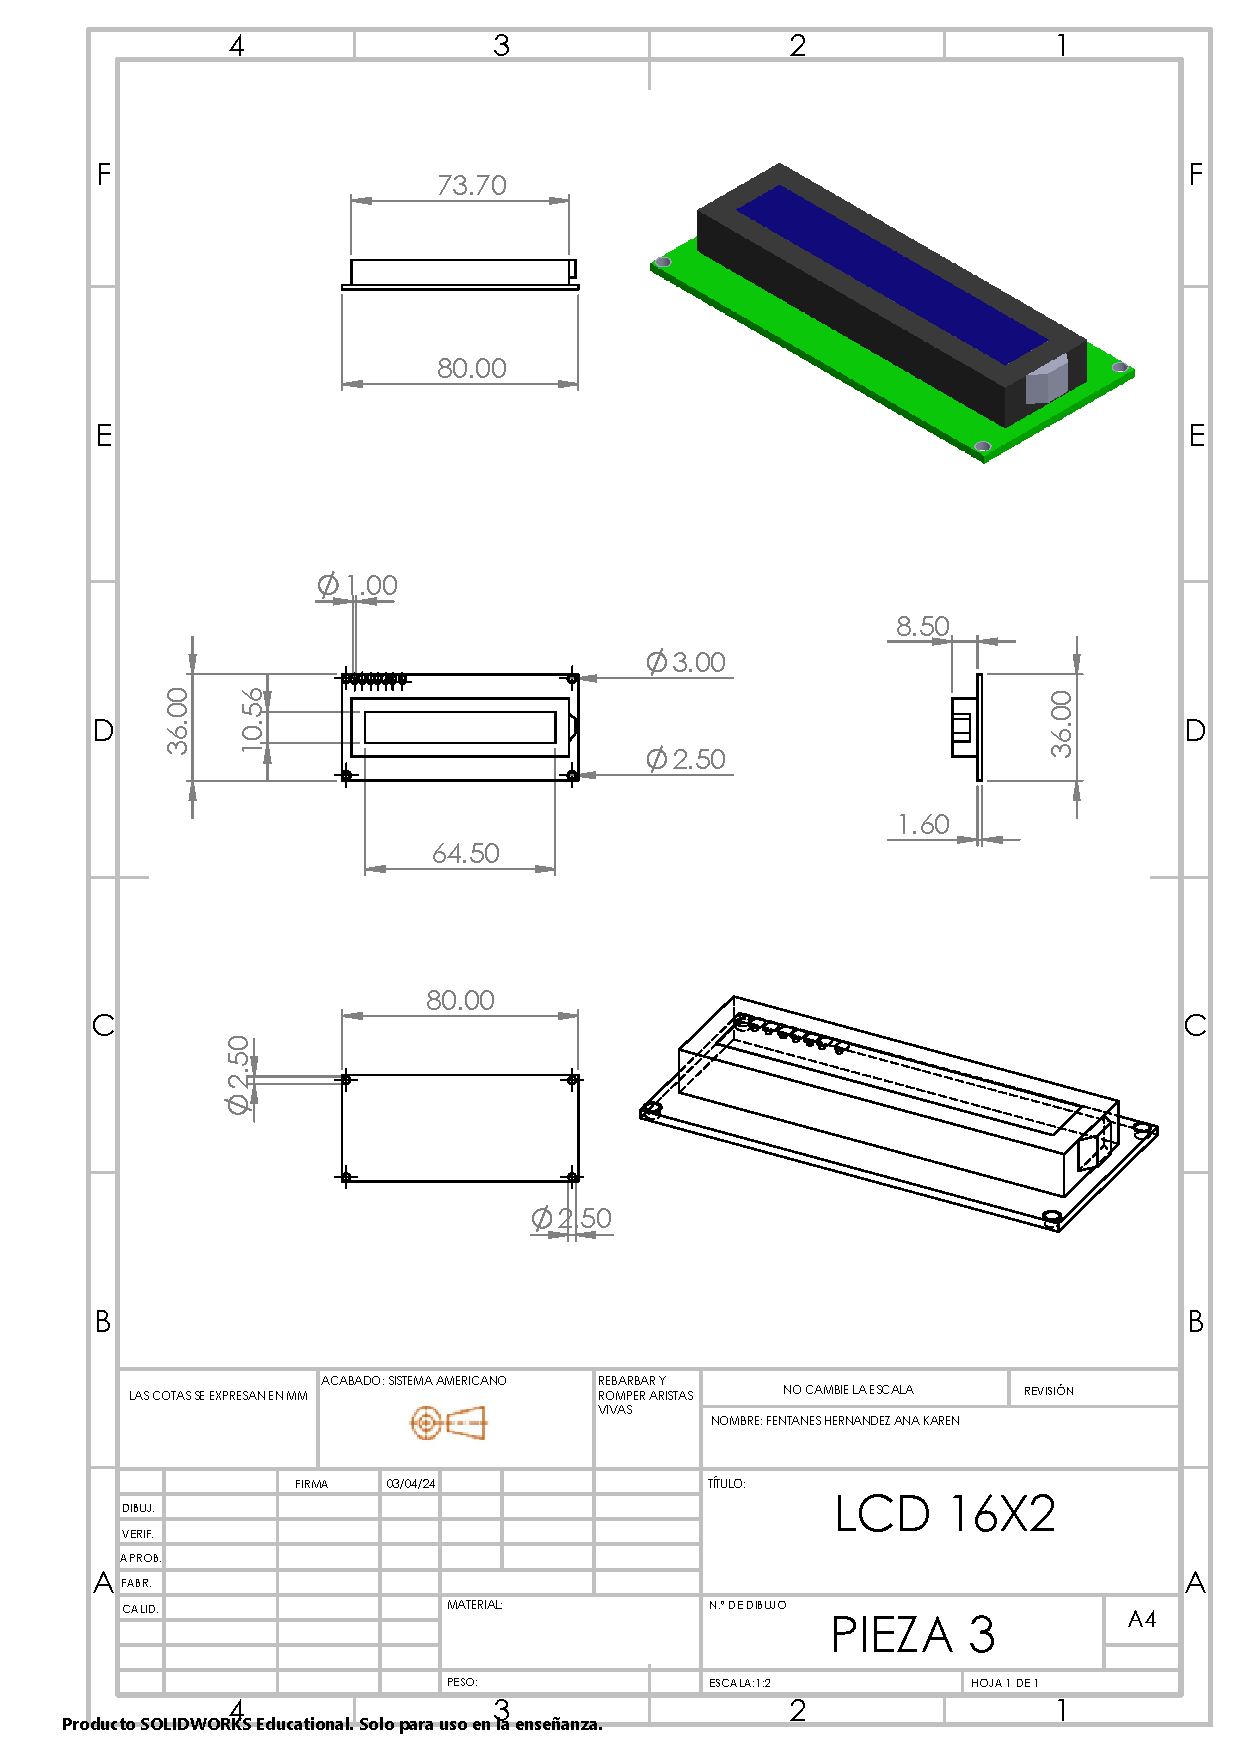
\includepdf[pages=-]{13/img/planoLcd.pdf}
    %
    \centering{\section[\appendixautorefname{}]{APÉNDICE}}\label{anexo:PlanoPotenciometro}
    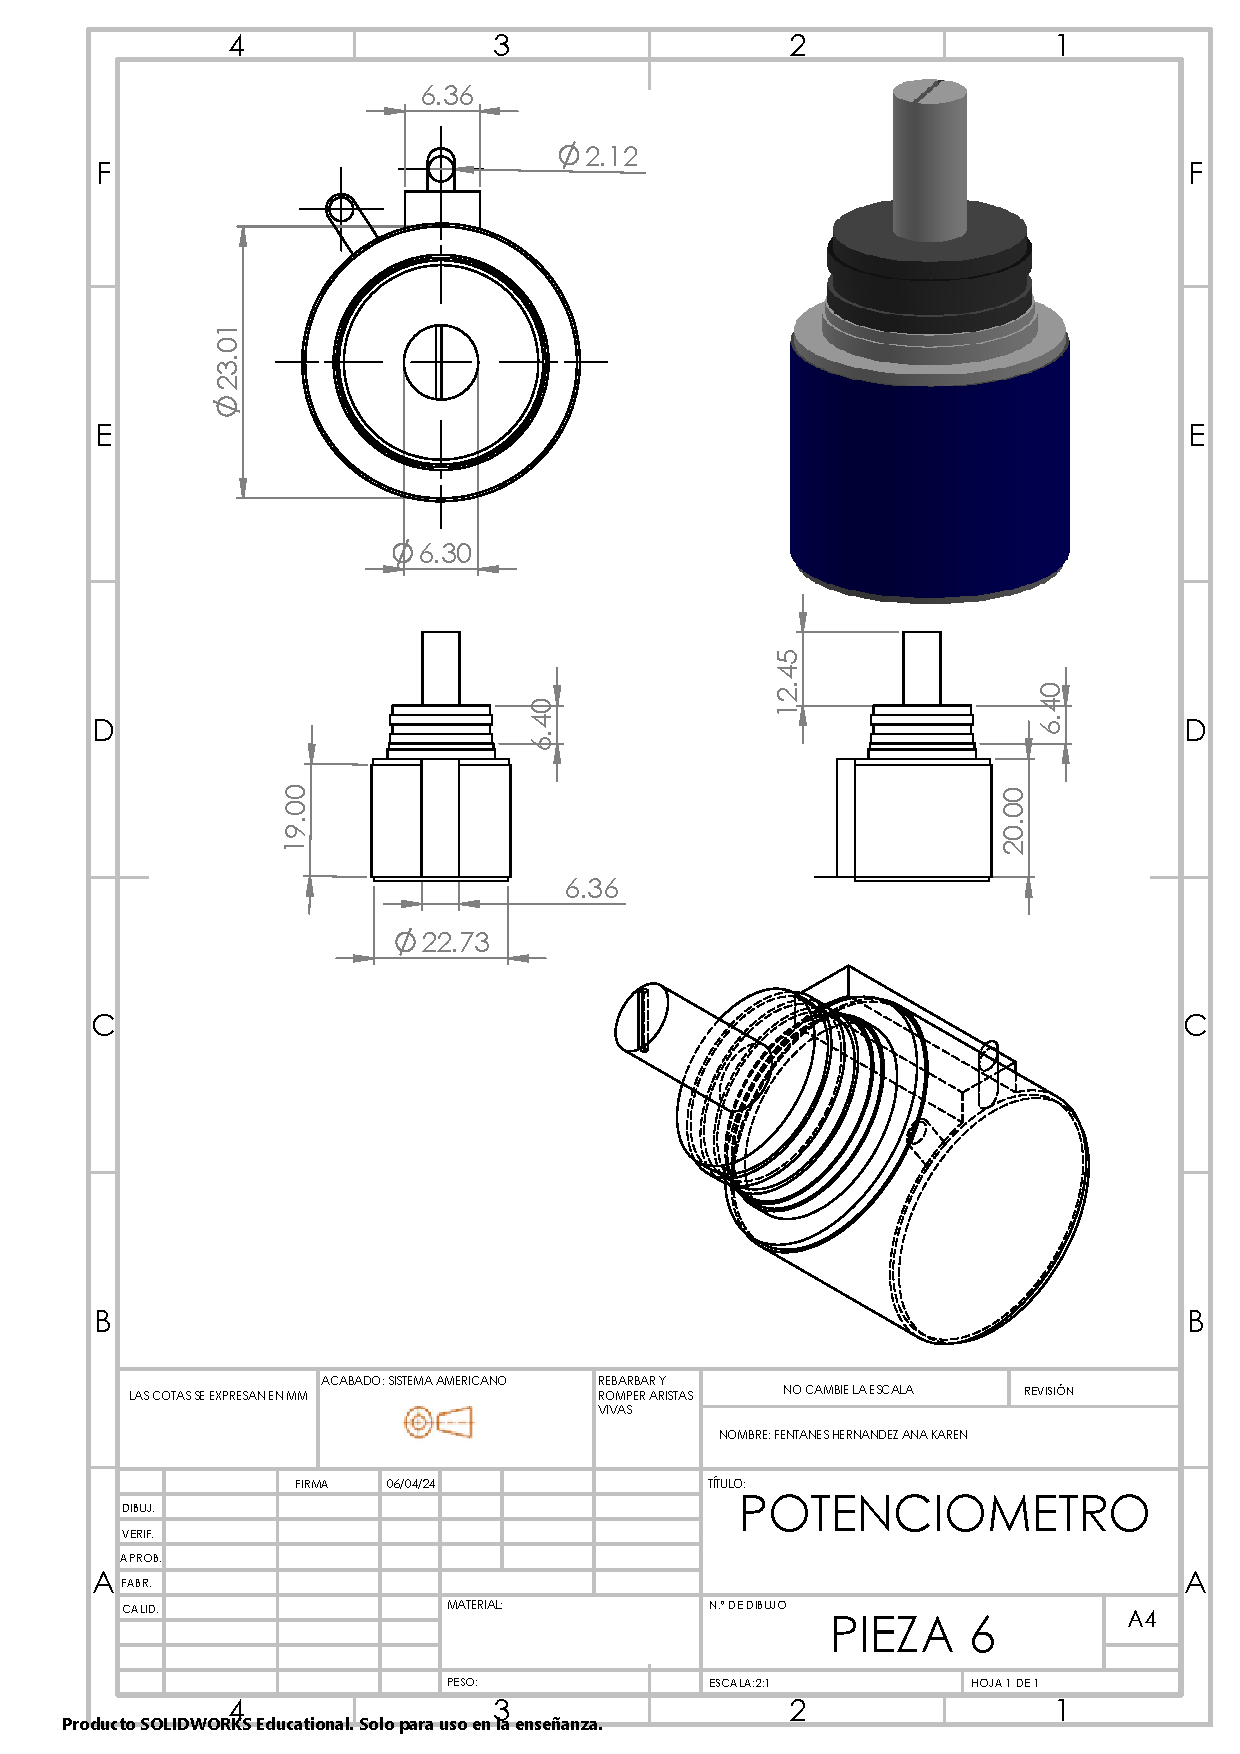
\includepdf[pages=-]{13/img/planoPotenciometro.pdf}
    %
    \centering{\section[\appendixautorefname{}]{APÉNDICE}}\label{anexo:PlanoResistencia}
    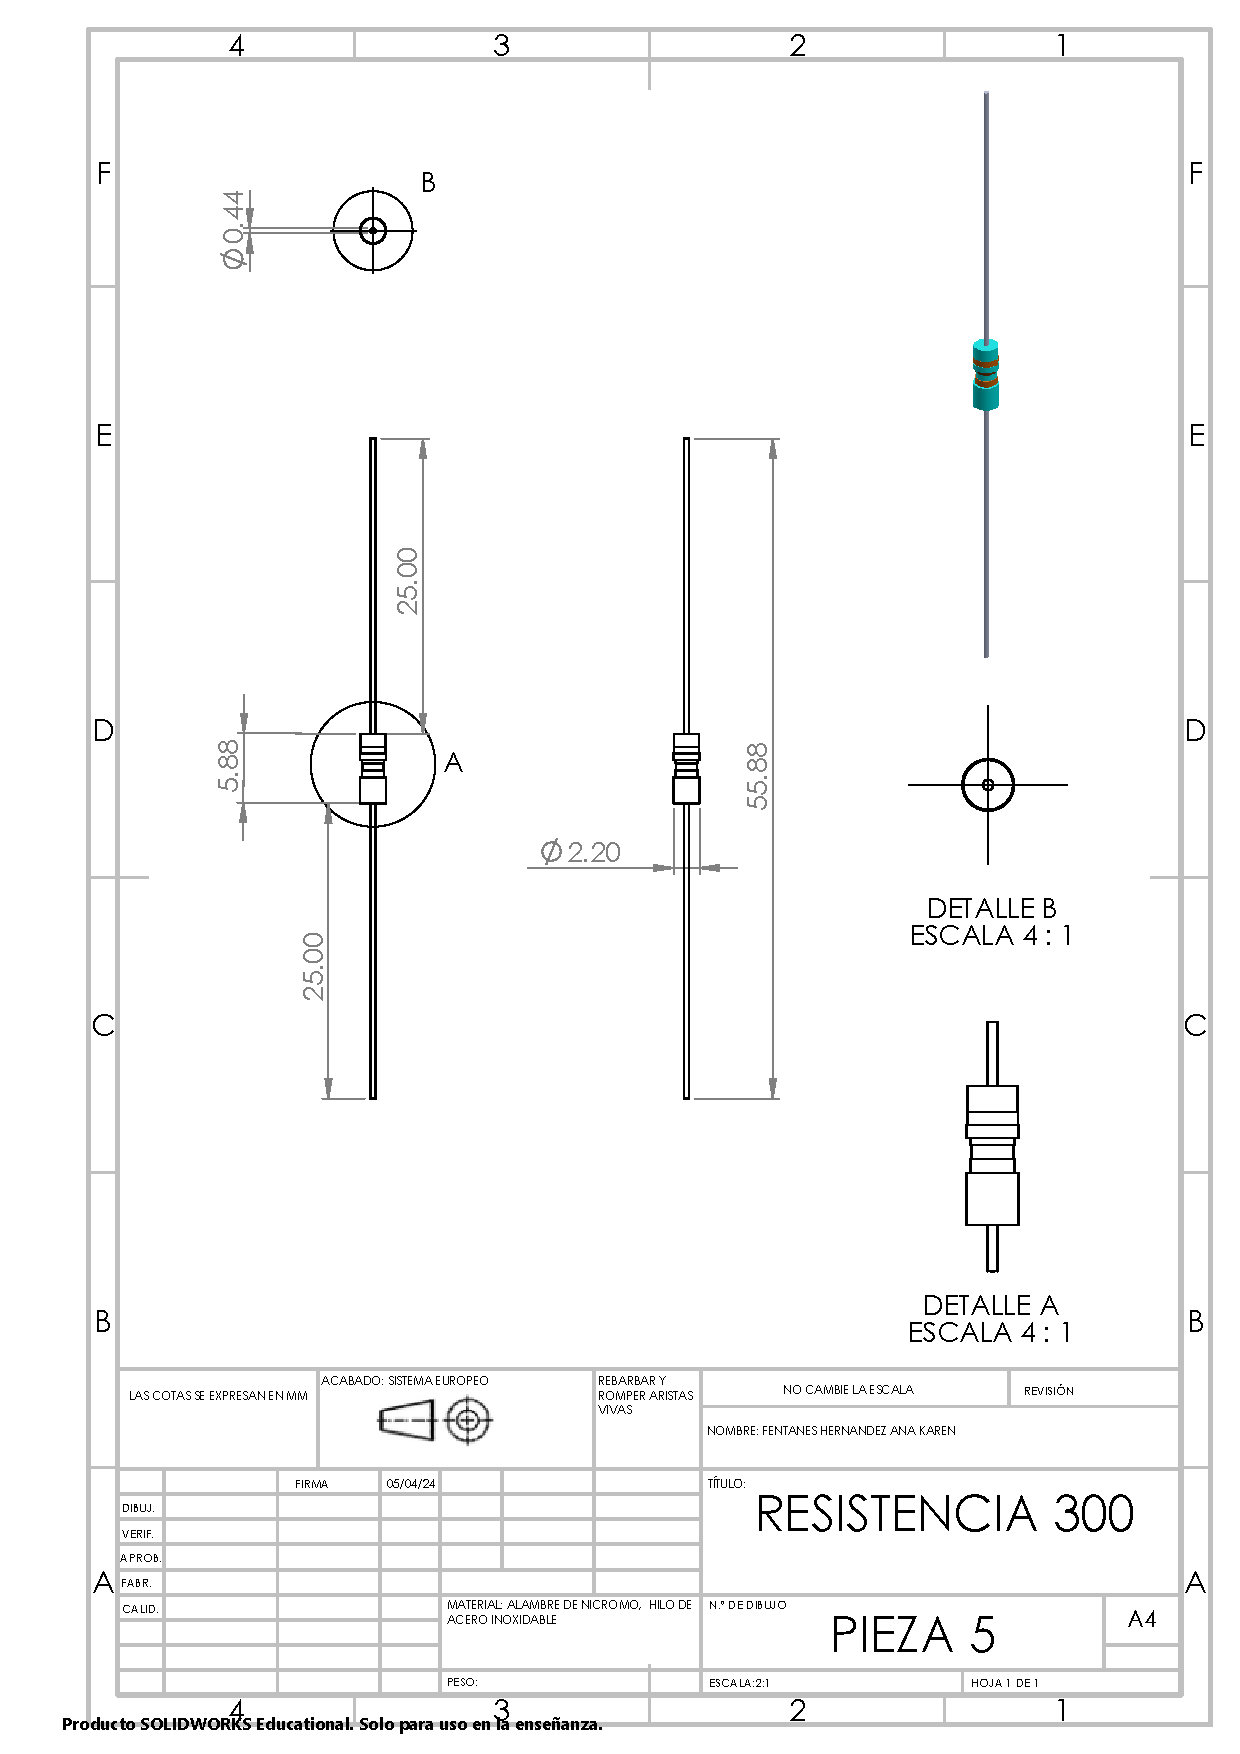
\includepdf[pages=-]{13/img/planoResistencia.pdf}
    
    %
    \centering{\section[\appendixautorefname{}]{APÉNDICE}}\label{anexo:ensambleCircuitoElectrónicoESP32-C6.pdf}
    \includepdf[pages=-]{13/img/ensambleCircuitoElectrónicoESP32-C6.pdf}
    
    %%%%%%%%%%%%%%%%%%%%%%%%%%%%%%%%%%%%%%%%